\section{Введение и основные определения.}
\subsection{Классическое и геометрическое определение вероятности.}
\subsubsection{Задача о разделе ставки (постановки Пачолли и Ферма).}
\noindent Рассмотрим первую задачу, которую можно связать с теорией вероятности. Данная задача была рассмотрена Лукой Пачолли в XV веке. Поставим её. 

\begin{problem}[О разделе ставки, постановка Пачолли]
    Два лучника решили посоревноваться в меткости и сделали некую ставку. Также, лучники договорились, что сумму забирает тот, кто первый выиграет 6 парных дуэлей. На счёте 5:3 соревнование прекратилось. Вопрос состоит в том, как поделить имеющуюся сумму. 
\end{problem}

\noindent В своём труде <<Об отношениях и пропорциях>> Пачолли предложил поделить имеющуюся ставку пропорционально счёту: 5 частей одному лучнику и 3 части другому. Верность данного решения не будет обсуждаться, так как для этого нужна корректная постановка задачи. 

\noindent С течением времени люди приближались к знакомым нам определениям, связанным с определением вероятности. 

\begin{definition}[Классическое]
    Пусть $\Omega = \{\omega_1, \dots, \omega_n\}$ ~---~ конечное множество взаимоисключающих равновозможных исходов, $A \subset \Omega$ ~---~ событие. Тогда вероятность события $A$ будет определяться как: $\P\{A\} = \frac{|A|}{|\Omega|}$.
\end{definition}

\noindent Существенным продвижением было появление геометрического определения вероятности, которое значительно облегчило работу с бесконечным количеством исходов. При определении геометрической вероятности часто пользуются постановкой <<бросаем точку на удачу>>. То есть с какой вероятностью точка, брошенная в фигуру $\Omega$ попадет в подмножество $A$. 

\begin{figure}[ht]
    
    \centering
    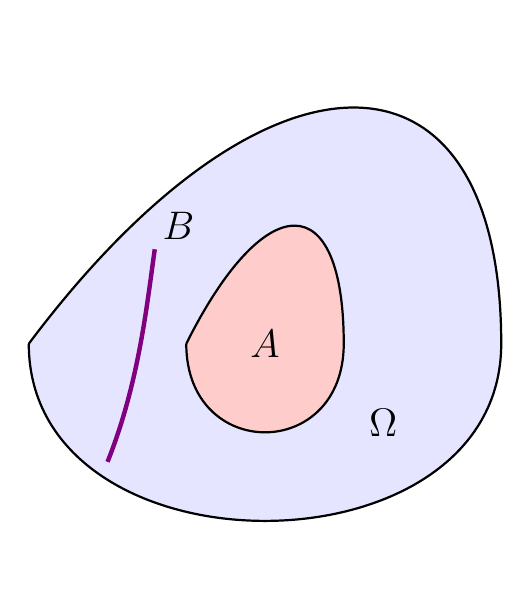
\begin{tikzpicture}
    
                % Главное множество
        \begin{scope}
          \clip (0,0) .. controls (3,4) and (6,4) .. (6,0)
                .. controls (6,-3) and (0,-3) .. (0,0);
          \fill[blue!10] (-1,-4) rectangle (7,5); % заливка множества
        \end{scope}
        
        % Подмножество
        \begin{scope}
          \clip (2,0) .. controls (3,2) and (4,2) .. (4,0)
                .. controls (4,-1.5) and (2,-1.5) .. (2,0);
          \fill[red!20] (-1,-4) rectangle (7,5); % заливка подмножества
        \end{scope}
        
        % Контуры множеств
        \draw[thick] (0,0) .. controls (3,4) and (6,4) .. (6,0)
                     .. controls (6,-3) and (0,-3) .. (0,0);
                     
        \draw[thick] (2,0) .. controls (3,2) and (4,2) .. (4,0)
                     .. controls (4,-1.5) and (2,-1.5) .. (2,0);
        
       \draw[violet, ultra thick] (1.0,-1.5) .. controls (1.4,-0.5) and (1.5,0.5) .. (1.6,1.2);
        \node at (1.9, 1.5) {\Large $B$};
        
        % Метки A и Omega
        \node at (3,0) {\Large $A$};
        \node at (4.5,-1) {\Large $\Omega$};
    
    \end{tikzpicture}
    \caption{Геометрическое определение вероятности}
\end{figure}

\begin{definition}[Геометрическое]
    Пусть $\Omega$ ~---~ измеримое множество, $A \subset \Omega$ ~---~ тоже измеримое множество. Тогда вероятность попадания в множество $A$ можем определить как $\P \{A\} = \frac{\mu(A)}{\mu(\Omega)}$
\end{definition}

\noindent Вместе с определением вероятности для множеств бесконечной мощности, это определение дает возможность работать с множествами нулевой меры, таких как линия $B$ на рисунке выше. 

\subsubsection{Парадокс Монти-Холла.}
\begin{problem}
    У игрока есть три шкатулки. В одной из шкатулок лежит приз. Игроку предлагается выбрать одну из них. После этого, ведущий показывает, что одна из двух оставшихся шкатулок пустая и предлагает поменять свой выбор. Соответственно, игрок может остаться с текущей шкатулкой, либо поменять свой выбор на оставшуюся. 
\end{problem}

\noindent Парадокс заключается в том, что изначально у игрока все три коробки равновероятные на выигрыш, то есть он заберет приз с вероятностью равной $\frac{1}{3}$. Посчитаем вероятности, которые получаются, после открытия шкатулки без приза. 

\begin{table}[h]
    \centering
    \begin{tabular}{|c|c|c|}
    \hline
    + & + &   \\ 
    \hline
    + &   & + \\ 
    \hline
      & + & + \\ 
    \hline
    \end{tabular}
    \caption{Расположение приза и выбор игрока}
\end{table}

\noindent Посмотрим на таблицу выше. По строкам мы отложили выбор человека, а по столбцам нахождение приза. Плюсами же обозначим ситуации, которые будут выигрышными, если поменять выбранную коробку. Исходя из классического определения вероятности, получаем, что с вероятностью равной $P\{\text{выигрыш}\} = \frac{6}{9} = \frac{2}{3}$ выгоднее менять выбранную коробку. 

\subsubsection{Парадокс Бертрана.}

\begin{problem}
    Пусть имеется окружность с радиусом $R$ и вписанный в неё треугольник. Необходимо определить вероятность того, что <<брошенная>> в данную окружность хорда окажется длиннее стороны треугольника. 
\end{problem}

\noindent Мы можем получить три разных ответа тремя разными способами. Данный парадокс иллюстрирует влияние того, как мы задаем пространство элементарных исходов, на получаемый ответ. 

\noindent Вариант 1. Зафиксируем треугольник и брошенную хорду так, чтобы хорда была параллельно треугольнику. Если изначально хорда брошена не так, мы можем повернуть треугольник. Тогда, подходящие нам исходы будут соответствовать хордам, которые будут пересекать радиус, перпендикулярно проведенный к хорде, внутри треугольника. Тогда, из геометрии полученная вероятность $P_1 = \frac{R/2}{R} = \frac{1}{2}$.

\noindent Вариант 2. Будем задавать расположение хорды углом, отсчитываемым от касательной к одному из углов. Тогда подходящие нам хорды будут иметь координаты от $\ang{60}$ до $\ang{120}$. Получившаяся вероятность события будет равна $P_2 = \frac{\ang{120} - \ang{60}}{\ang{180}} = \frac{1}{3}$

\noindent Вариант 3. Будем бросать на удачу точку, являющуюся центром нашей хорды. Заметим, что удачные исходы в таком случае будут задаваться окружностью, вписанной в треугольник. Тогда искомая вероятность будет равна $P_2 = \frac{\pi (R/2)^2}{\pi R^2} = \frac{1}{4}$. 

\begin{figure}[H]
    \centering
    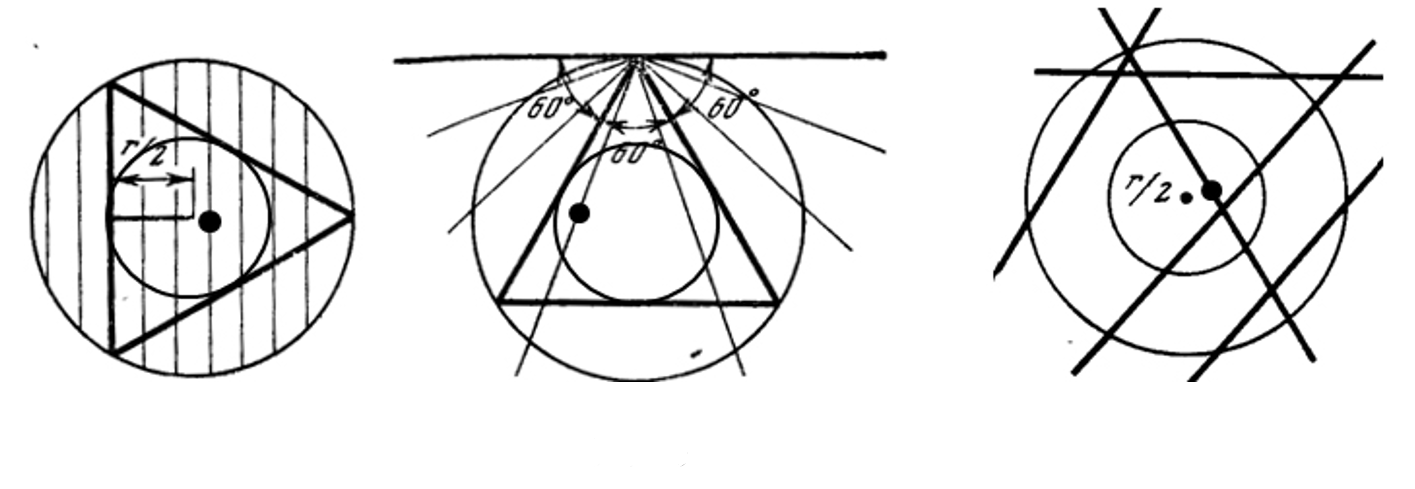
\includegraphics[width=0.5\linewidth]{exam/pictures/bertran.png}
    \caption{1, 2 и 3 вариант соответственно}
\end{figure}
